% ============================================================================
% CHƯƠNG 2: MÔ HÌNH LẬP TRÌNH CUDA
% ============================================================================
\chapter{Mô hình Lập trình CUDA}
\label{chap:cuda_basics}

\section{Kiến trúc GPU NVIDIA}

\subsection{Streaming Multiprocessor (SM)}

GPU NVIDIA được tổ chức thành nhiều \textbf{Streaming Multiprocessor (SM)}. Mỗi SM chứa:
\begin{itemize}
    \item \textbf{CUDA Cores (SP)}: Các đơn vị tính toán cơ bản
    \item \textbf{Shared Memory}: Bộ nhớ chia sẻ tốc độ cao (48-96 KB)
    \item \textbf{Register File}: Thanh ghi cho threads
    \item \textbf{Warp Scheduler}: Bộ lập lịch thực thi
\end{itemize}

\begin{figure}[H]
\centering
\begin{tikzpicture}[scale=0.85]
    % Main GPU box
    \draw[thick, fill=gray!10, rounded corners] (0,0) rectangle (14,9);
    \node[font=\bfseries\large] at (7,8.5) {NVIDIA GPU (Tesla T4)};
    
    % SMs
    \foreach \i in {0,1,2,3} {
        \foreach \j in {0,1} {
            \pgfmathtruncatemacro{\smnum}{\i*2+\j}
            \draw[fill=cudablue!20, rounded corners] 
                ({1+\i*3}, {1+\j*3.5}) rectangle ({3.5+\i*3}, {4+\j*3.5});
            \node[font=\footnotesize\bfseries] at ({2.25+\i*3}, {3.7+\j*3.5}) {SM \smnum};
            
            % CUDA cores grid
            \foreach \x in {0,1,2,3} {
                \foreach \y in {0,1,2,3} {
                    \fill[cudagreen!70] ({1.2+\i*3+\x*0.25}, {1.3+\j*3.5+\y*0.25}) 
                        rectangle ++(0.2,0.2);
                }
            }
            
            % Shared memory
            \draw[fill=orange!40] ({2.4+\i*3}, {1.2+\j*3.5}) rectangle ({3.3+\i*3}, {2.5+\j*3.5});
            \node[font=\tiny, align=center] at ({2.85+\i*3}, {1.85+\j*3.5}) {Shared\\Mem};
            
            % Registers
            \draw[fill=purple!30] ({1.2+\i*3}, {2.8+\j*3.5}) rectangle ({3.3+\i*3}, {3.4+\j*3.5});
            \node[font=\tiny] at ({2.25+\i*3}, {3.1+\j*3.5}) {Registers};
        }
    }
    
    % Legend
    \fill[cudagreen!70] (0.5,0.3) rectangle ++(0.3,0.3);
    \node[right, font=\tiny] at (0.9,0.45) {CUDA Core};
    
    \fill[orange!40] (3,0.3) rectangle ++(0.5,0.3);
    \node[right, font=\tiny] at (3.6,0.45) {Shared Memory};
    
    \fill[purple!30] (6,0.3) rectangle ++(0.5,0.3);
    \node[right, font=\tiny] at (6.6,0.45) {Registers};
\end{tikzpicture}
\caption{Kiến trúc GPU với nhiều Streaming Multiprocessors}
\label{fig:gpu_arch}
\end{figure}

\subsection{Mô hình SIMT (Single Instruction Multiple Thread)}

GPU thực thi theo mô hình \textbf{SIMT} (Single Instruction Multiple Thread):
\begin{itemize}
    \item Các thread được nhóm thành \textbf{warps} (32 threads/warp)
    \item Tất cả threads trong một warp thực thi cùng một instruction
    \item \textbf{Warp divergence}: Khi có branch (if-else), các threads khác nhau có thể đi theo các nhánh khác nhau, gây giảm hiệu năng
\end{itemize}

\section{Hệ thống phân cấp Thread}

CUDA tổ chức threads theo hệ thống phân cấp 3 cấp:

\begin{figure}[H]
\centering
\begin{tikzpicture}[
    gridbox/.style={draw, thick, fill=blue!10, minimum width=8cm, minimum height=2cm, rounded corners},
    blockbox/.style={draw, thick, fill=green!10, minimum width=2cm, minimum height=1.2cm, rounded corners},
    threadbox/.style={draw, fill=yellow!20, minimum width=0.4cm, minimum height=0.4cm}
]
    % Grid
    \node[gridbox, minimum height=5cm] (grid) at (0,0) {};
    \node[font=\bfseries, above] at (0,2.5) {GRID};
    
    % Blocks
    \foreach \i/\x in {0/-2.5, 1/0, 2/2.5} {
        \node[blockbox] (block\i) at (\x, 0.8) {};
        \node[font=\footnotesize] at (\x, 1.5) {Block (\i,0)};
        
        % Threads in each block
        \foreach \tx in {0,1,2,3} {
            \foreach \ty in {0,1} {
                \node[threadbox] at ({\x-0.7+\tx*0.45}, {0.4+\ty*0.5}) {};
            }
        }
    }
    
    \foreach \i/\x in {0/-2.5, 1/0, 2/2.5} {
        \node[blockbox] (block\i b) at (\x, -1.2) {};
        \node[font=\footnotesize] at (\x, -0.5) {Block (\i,1)};
        
        \foreach \tx in {0,1,2,3} {
            \foreach \ty in {0,1} {
                \node[threadbox] at ({\x-0.7+\tx*0.45}, {-1.6+\ty*0.5}) {};
            }
        }
    }
    
    % Annotations
    \draw[<->, thick, red] (5,2.5) -- (5,-2.5) node[midway, right, font=\footnotesize] {gridDim.y = 2};
    \draw[<->, thick, red] (-4.5,3) -- (4.5,3) node[midway, above, font=\footnotesize] {gridDim.x = 3};
    
    % Block detail
    \node[font=\bfseries] at (8,2) {Chi tiết Block:};
    \draw[thick, fill=green!10, rounded corners] (6.5,0) rectangle (9.5,1.5);
    \foreach \tx in {0,1,2,3} {
        \foreach \ty in {0,1} {
            \draw[fill=yellow!30] ({6.8+\tx*0.7}, {0.3+\ty*0.5}) rectangle ++(0.5,0.4);
            \node[font=\tiny] at ({7.05+\tx*0.7}, {0.5+\ty*0.5}) {t\tx,\ty};
        }
    }
    \node[font=\footnotesize] at (8, -0.3) {blockDim = (4, 2)};
    
\end{tikzpicture}
\caption{Hệ thống phân cấp Grid - Block - Thread}
\label{fig:thread_hierarchy}
\end{figure}

\subsection{Biến tích hợp (Built-in Variables)}

CUDA cung cấp các biến tích hợp để xác định vị trí của mỗi thread:

\begin{table}[H]
\centering
\caption{Các biến tích hợp trong CUDA}
\label{tab:builtin_vars}
\begin{tabular}{@{}lp{8cm}@{}}
\toprule
\textbf{Biến} & \textbf{Mô tả} \\
\midrule
\code{threadIdx.x/y/z} & Chỉ số thread trong block (local index) \\
\code{blockIdx.x/y/z} & Chỉ số block trong grid \\
\code{blockDim.x/y/z} & Kích thước block (số threads/chiều) \\
\code{gridDim.x/y/z} & Kích thước grid (số blocks/chiều) \\
\bottomrule
\end{tabular}
\end{table}

\subsection{Tính chỉ số global}

Công thức tính chỉ số global của thread trong mảng 1D và 2D:

\textbf{1D Array:}
\begin{equation}
\text{globalIdx} = \text{blockIdx.x} \times \text{blockDim.x} + \text{threadIdx.x}
\end{equation}

\textbf{2D Array (Row-major):}
\begin{equation}
\begin{aligned}
\text{ix} &= \text{blockIdx.x} \times \text{blockDim.x} + \text{threadIdx.x} \\
\text{iy} &= \text{blockIdx.y} \times \text{blockDim.y} + \text{threadIdx.y} \\
\text{idx} &= \text{iy} \times \text{width} + \text{ix}
\end{aligned}
\end{equation}

\begin{figure}[H]
\centering
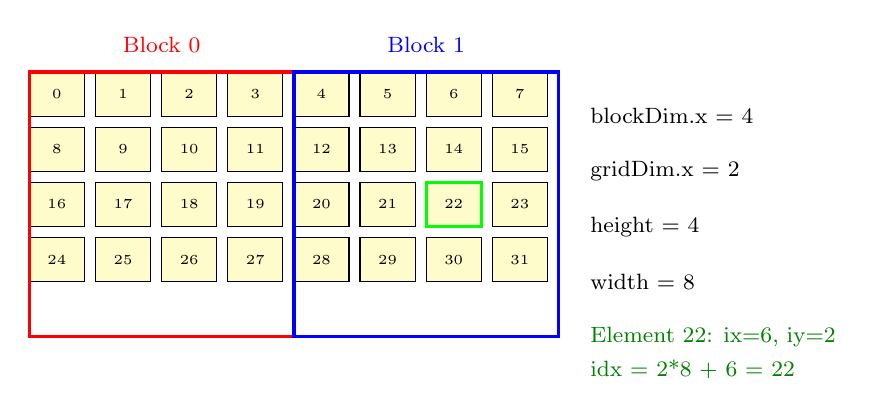
\begin{tikzpicture}[scale=0.7]
    % Grid of elements
    \foreach \i in {0,...,7} {
        \foreach \j in {0,...,3} {
            \pgfmathtruncatemacro{\idx}{\j*8+\i}
            \draw[fill=yellow!20] (\i*1.2, -\j*1) rectangle ++(1,0.8);
            \node[font=\tiny] at ({\i*1.2+0.5}, {-\j*1+0.4}) {\idx};
        }
    }
    
    % Block boundaries
    \draw[very thick, red] (0,-4) rectangle (4.8,0.8);
    \draw[very thick, blue] (4.8,-4) rectangle (9.6,0.8);
    
    \node[red, font=\footnotesize] at (2.4, 1.3) {Block 0};
    \node[blue, font=\footnotesize] at (7.2, 1.3) {Block 1};
    
    % Formula explanation
    \node[right, font=\footnotesize] at (10, 0) {blockDim.x = 4};
    \node[right, font=\footnotesize] at (10, -1) {gridDim.x = 2};
    \node[right, font=\footnotesize] at (10, -2) {height = 4};
    \node[right, font=\footnotesize] at (10, -3) {width = 8};
    
    % Highlight specific element
    \draw[very thick, green] (6*1.2, -2*1) rectangle ++(1,0.8);
    \node[green!50!black, font=\footnotesize, right] at (10, -4) {Element 22: ix=6, iy=2};
    \node[green!50!black, font=\footnotesize, right] at (10, -4.6) {idx = 2*8 + 6 = 22};
    
\end{tikzpicture}
\caption{Ánh xạ 2D Block/Thread vào mảng 1D}
\label{fig:2d_indexing}
\end{figure}

\section{Mô hình bộ nhớ CUDA}

\subsection{Các loại bộ nhớ}

CUDA cung cấp nhiều loại bộ nhớ với đặc điểm khác nhau:

\begin{figure}[H]
\centering
\begin{tikzpicture}[
    membox/.style={draw, thick, rounded corners, minimum width=3cm, minimum height=1cm, font=\footnotesize},
    arrow/.style={->, thick}
]
    % Device (GPU)
    \draw[thick, fill=gray!5, rounded corners] (0,0) rectangle (12,8);
    \node[font=\bfseries] at (6,7.5) {GPU Device};
    
    % Global Memory
    \draw[fill=red!20, rounded corners] (0.5,0.5) rectangle (11.5,1.8);
    \node[font=\bfseries\footnotesize] at (6,1.15) {Global Memory (VRAM) - Chậm, Lớn (GB)};
    
    % Constant Memory
    \draw[fill=purple!20, rounded corners] (0.5,2) rectangle (5,3);
    \node[font=\footnotesize] at (2.75,2.5) {Constant Memory (64KB)};
    
    % Texture Memory
    \draw[fill=purple!20, rounded corners] (5.5,2) rectangle (11.5,3);
    \node[font=\footnotesize] at (8.5,2.5) {Texture Memory (Cached)};
    
    % SM 0
    \draw[fill=blue!10, rounded corners] (0.5,3.5) rectangle (5.5,7);
    \node[font=\bfseries\footnotesize] at (3,6.7) {SM 0};
    
    % Shared Memory in SM0
    \draw[fill=orange!30, rounded corners] (0.7,5.5) rectangle (5.3,6.4);
    \node[font=\footnotesize] at (3,5.95) {Shared Memory (48KB)};
    
    % Registers in SM0
    \draw[fill=green!30, rounded corners] (0.7,4.5) rectangle (2.5,5.3);
    \node[font=\tiny] at (1.6,4.9) {Registers};
    \draw[fill=green!30, rounded corners] (2.7,4.5) rectangle (4.5,5.3);
    \node[font=\tiny] at (3.6,4.9) {Registers};
    
    % Local Memory indicator
    \draw[fill=yellow!30, rounded corners] (0.7,3.7) rectangle (5.3,4.3);
    \node[font=\tiny] at (3,4) {Local Memory (per thread, in DRAM)};
    
    % SM 1 (simplified)
    \draw[fill=blue!10, rounded corners] (6,3.5) rectangle (11.5,7);
    \node[font=\bfseries\footnotesize] at (8.75,6.7) {SM 1};
    \draw[fill=orange!30, rounded corners] (6.2,5.5) rectangle (11.3,6.4);
    \node[font=\footnotesize] at (8.75,5.95) {Shared Memory (48KB)};
    
    % Legend
    \node[font=\footnotesize] at (6,-0.5) {Tốc độ: Registers > Shared > Constant/Texture (cached) > Global/Local};
    
\end{tikzpicture}
\caption{Hệ thống phân cấp bộ nhớ GPU}
\label{fig:memory_hierarchy}
\end{figure}

\begin{table}[H]
\centering
\caption{So sánh các loại bộ nhớ CUDA}
\label{tab:memory_comparison}
\begin{tabular}{@{}lcccl@{}}
\toprule
\textbf{Loại} & \textbf{Phạm vi} & \textbf{Tốc độ} & \textbf{Dung lượng} & \textbf{Khai báo} \\
\midrule
Register & Thread & Rất nhanh & KB/thread & Biến cục bộ \\
Shared & Block & Nhanh & 48-96 KB & \code{\_\_shared\_\_} \\
Global & Grid/Host & Chậm & GB & \code{cudaMalloc()} \\
Constant & Grid & Nhanh (cached) & 64 KB & \code{\_\_constant\_\_} \\
Local & Thread & Chậm & Tùy chỉnh & Mảng lớn cục bộ \\
\bottomrule
\end{tabular}
\end{table}

\subsection{Các hàm quản lý bộ nhớ}

\begin{lstlisting}[caption={Các hàm quản lý bộ nhớ CUDA}, label={lst:memory_funcs}]
// Cap phat bo nho tren GPU
cudaMalloc((void**)&d_ptr, size_in_bytes);

// Giai phong bo nho
cudaFree(d_ptr);

// Copy du lieu Host -> Device
cudaMemcpy(d_ptr, h_ptr, size, cudaMemcpyHostToDevice);

// Copy du lieu Device -> Host
cudaMemcpy(h_ptr, d_ptr, size, cudaMemcpyDeviceToHost);

// Copy du lieu Device -> Device
cudaMemcpy(d_dst, d_src, size, cudaMemcpyDeviceToDevice);

// Khoi tao bo nho voi gia tri 0
cudaMemset(d_ptr, 0, size_in_bytes);
\end{lstlisting}

\section{Đồng bộ hóa}

\subsection{Đồng bộ trong Block}

Hàm \code{\_\_syncthreads()} đảm bảo tất cả threads trong block đã hoàn thành công việc trước khi tiếp tục:

\begin{lstlisting}[caption={Sử dụng \_\_syncthreads()}, label={lst:syncthreads}]
__global__ void kernelWithSync(float *data) {
    __shared__ float sharedData[256];
    
    // Moi thread load du lieu vao shared memory
    sharedData[threadIdx.x] = data[blockIdx.x * blockDim.x + threadIdx.x];
    
    // Cho tat ca threads hoan thanh load
    __syncthreads();
    
    // Bay gio co the truy cap an toan sharedData cua cac thread khac
    if (threadIdx.x > 0) {
        float neighbor = sharedData[threadIdx.x - 1];
        // ... xu ly ...
    }
}
\end{lstlisting}

\subsection{Đồng bộ Grid}

\code{cudaDeviceSynchronize()} chờ GPU hoàn thành tất cả công việc trước khi CPU tiếp tục:

\begin{lstlisting}[caption={Đồng bộ Host-Device}]
kernel<<<grid, block>>>(d_data);
cudaDeviceSynchronize();  // Cho kernel hoan thanh
// Bay gio co the copy ket qua ve Host an toan
cudaMemcpy(h_data, d_data, size, cudaMemcpyDeviceToHost);
\end{lstlisting}

\section{Đo thời gian thực thi}

\subsection{Sử dụng CUDA Events}

CUDA Events là cách chính xác nhất để đo thời gian kernel:

\begin{lstlisting}[caption={Đo thời gian với CUDA Events}, label={lst:cuda_events}]
cudaEvent_t start, stop;
cudaEventCreate(&start);
cudaEventCreate(&stop);

// Bat dau do thoi gian
cudaEventRecord(start);

// Chay kernel
myKernel<<<grid, block>>>(d_data);

// Ket thuc do thoi gian
cudaEventRecord(stop);
cudaEventSynchronize(stop);

// Tinh thoi gian (milliseconds)
float milliseconds = 0;
cudaEventElapsedTime(&milliseconds, start, stop);
printf("Kernel time: %.4f ms\n", milliseconds);

// Giai phong events
cudaEventDestroy(start);
cudaEventDestroy(stop);
\end{lstlisting}

\section{Cấu hình Kernel tối ưu}

\subsection{Chọn Block Size}

Block size ảnh hưởng đến:
\begin{itemize}
    \item \textbf{Occupancy}: Tỷ lệ sử dụng SM
    \item \textbf{Register pressure}: Số registers mỗi thread sử dụng
    \item \textbf{Shared memory}: Dung lượng shared memory mỗi block
\end{itemize}

\textbf{Nguyên tắc chung:}
\begin{itemize}
    \item Block size nên là bội số của 32 (warp size): 128, 256, 512
    \item Thử nghiệm với nhiều giá trị để tìm cấu hình tối ưu
    \item Sử dụng \code{cudaOccupancyMaxPotentialBlockSize()} để tự động chọn
\end{itemize}

\begin{table}[H]
\centering
\caption{Ảnh hưởng của Block Size đến hiệu năng (ví dụ)}
\label{tab:blocksize_perf}
\begin{tabular}{@{}cccc@{}}
\toprule
\textbf{Block Size} & \textbf{Blocks/SM} & \textbf{Occupancy} & \textbf{Time (ms)} \\
\midrule
32 & 32 & 50\% & 5.2 \\
64 & 16 & 50\% & 4.8 \\
128 & 8 & 50\% & 3.2 \\
256 & 4 & 50\% & 2.9 \\
512 & 2 & 50\% & 3.1 \\
1024 & 1 & 50\% & 4.5 \\
\bottomrule
\end{tabular}
\end{table}

\section{Kết luận chương}

Chương này đã trình bày các khái niệm cốt lõi của mô hình lập trình CUDA:

\begin{itemize}
    \item \textbf{Kiến trúc GPU}: SM, CUDA cores, và mô hình SIMT
    \item \textbf{Thread hierarchy}: Grid $\rightarrow$ Block $\rightarrow$ Thread
    \item \textbf{Memory hierarchy}: Register $\rightarrow$ Shared $\rightarrow$ Global
    \item \textbf{Đồng bộ hóa}: \code{\_\_syncthreads()} và \code{cudaDeviceSynchronize()}
    \item \textbf{Đo thời gian}: CUDA Events cho kết quả chính xác
\end{itemize}

Hiểu rõ các khái niệm này là nền tảng để phát triển các ứng dụng CUDA hiệu quả trong các chương tiếp theo.
